\subsection{Risk management}
\begin{landscape}
	\rowcolors{1}{gray!25}{white}
	\begin{longtable}[H]
		{l|p{0.22\textwidth}| p{0.3\textwidth} | p{0.1\textwidth} | p{0.1\textwidth} | p{0.3\textwidth} | p{0.3\textwidth}}
		
		\textbf{Nr} & \textbf{Title} & \textbf{Description} & 
		\textbf{Max Harm [h]} & \textbf{Proba- bility} & \textbf{Prevention} &  
		\textbf{Behaviour at entry}\\ \hline
		
		R1 & Underestimation of workload & One or more team members can't finish a feature in time or loses to much time for a minor feature & 120 & 25\% & Weekly scrum meetings with feedback about the current work progress. Estimate workload together. Include time reserve & Help each other, if one is struggling. Feature reduction at latest. \\ 
		
		R2 & Workflow is not working & Toolchain is not working as planed. The used components aren't ideal for the problem & 30 & 15\% & Use experience to get a good setup and test it alot in the beginning & Redefine toolchain or change single tool \\ 
		
		R3 & Communication problems & Team is not working together and each member is developing individual. Creating incompatible interfaces. Talking with the industrial partner isn't possible as expected, due to time difference or no enough time & 70 & 20\% & Weekly scrum meetings and agreements. Already worked in other projects as a team before & Increase written documentation and working closer together. Having a fixed meeting with the industrial partner \\ 
		
		R4 & Lack of knowledge & Team has to less knowledge about Dafny, VSCode and the development of a VSCode Plugin & 80 & 10\% & Already experience with typescript for plugin development, as preparatory work informed about Dafny & Find necessary knowledge online, get help from Microsoft Research \\ 
		
		R5 & Data lose or manipulation & Data lose because of a server crash or to open permissions to access and modify data & 20 & 3\% & Regularly backups and restrictive permissions to change files & Use backup to restore data. Extend safety measures \\ 
		
		R6 & Failure developer machine & One of the developer machines aren't working anymore. & 10 & 1\% & Limited, regularly commits and backups. & Switch temporary to the school computer and install the necessary tools. \\
		
		R7 & Implementing the DSL is to complicated to implement or to use & The DSL would be needed to suggest possible contracts or to customize the best practice. & 100 & 30\% & This core feature has to be looked carefully that it really fits our needs and that other developer can really use the plugin. & Read about DSL, talking to people which have already worked with it. \\
		
		R8 & Supporting all features on the different environments is not possible & Due to that Windows, OSX and Linux are quite different, it could be that some features aren't possible to implement on a platform or causes a big overhead to get it running & 10 & 25\% & Using as much of the standard api as possible. Implement specific features platform dependant. & Disable a certain feature on a platform or look for a workaround. \\	
		
		R9 & Automatic installer of Dafny is not possible & Maybe of security restrictions, it could be possible that you can't download and install additional software and setting environment variables. & 35 & 20\% & Test if downloading of software can done inside VS Code. & Automatic installer can't be done inside the plugin. Switch to a different strategy and implement an automatic installer over a additional executable, which could also install the plugin in vscode. \\
		
		\caption{Risk management}
		\label{tab:Risk management}
	\end{longtable}
\end{landscape}

\subsection{Risk Matrix}
\begin{figure}[H]
	\centering
	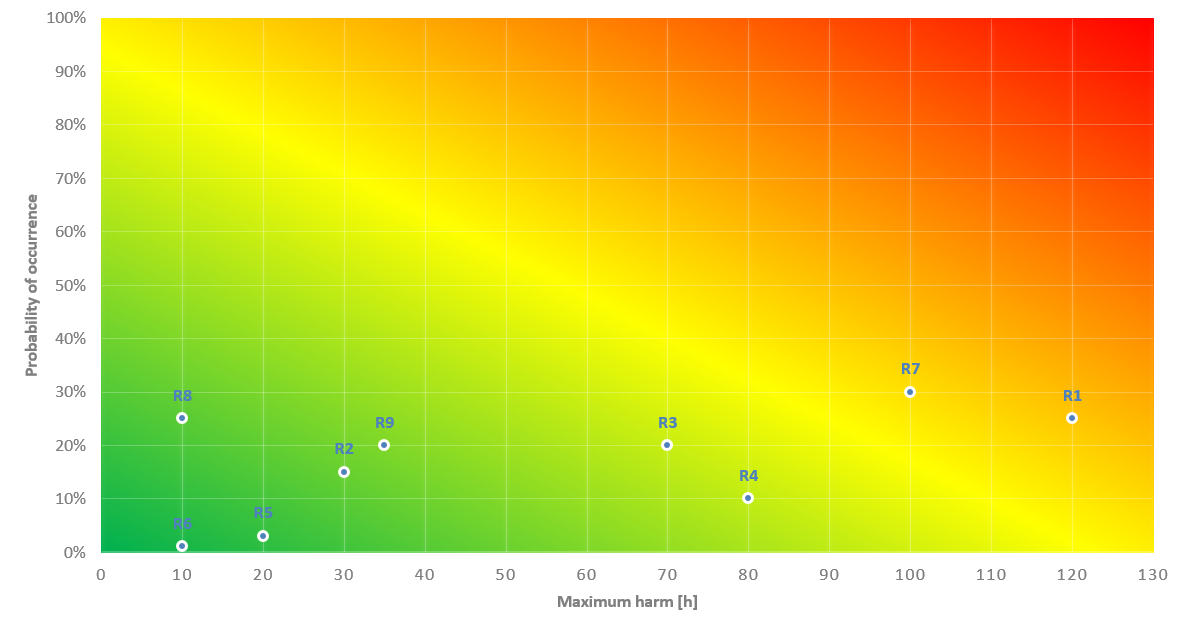
\includegraphics[width=1.2\textwidth]{img/riskmatrix}
	\caption{Risk Matrix}
	\label{fig:Risk Maxtrix}
\end{figure}
